\documentclass[xcolor=pdftex,dvipsnames]{beamer}

\usepackage{amsmath}
\usepackage{amssymb}

\usepackage{comment}
\usepackage{textcomp}

\title{Microeconomic Theory --- ECON 323 503 \\ Chapter 10: General
  Equilibrium and Economic Welfare}
\author{Vikram Manjunath}       %
\institute{Texas A\&M University}
\setbeamertemplate{navigation symbols}{}
\setbeamertemplate{footline}{}
\usefonttheme{serif}
\begin{document}

\maketitle

\begin{frame}
\frametitle{Outline}
\begin{enumerate}[<+->]
\item General Equilibrium: We can study all interrelated markets at
  once.
\item Trade between two people: Both benefit from mutually agreeable
  trades.
\item Competitive exchange:
  \begin{itemize}
  \item Allocation is efficient at a competitive equilibrium.
  \item Every efficient allocation is a competitive equilibrium for
    some initial distribution.
  \end{itemize}
\item  Efficiency and equity: Efficiency doesn't narrow down what
  allocations are good. Equity can be considered to do that.
\end{enumerate}
\end{frame}

\begin{frame}
  \frametitle{General Equilibrium}
  So far we studied economies with just one good. 

\uncover<2->{  \bigskip
  Trade-off was between consuming that good and having money to spend
  on other goods.}

\uncover<3->{    \bigskip
  This is ``partial equilibrium'' analysis.}

  \bigskip
\uncover<4->{    But how do changes in the market for one good affect the market for
  another good?}

  \bigskip
\uncover<5->{    To answer this, we use ``general equilibrium'' analysis.}

  \bigskip
\uncover<6->{    That is, we look at equilibrium in all markets simultaneously.}

\end{frame}


\begin{frame}
  \frametitle{Competitive equilibrium in two interrelated markets}
  Market for Good 1:
  \[
  \begin{array}{cc}
    D_1(p_1,p_2) & S_1(p_1)      
    \end{array}
  \]

\uncover<2->{    Market for Good 2:
  \[
  \begin{array}{cc}
    D_2(p_1,p_2) & S_2(p_2)      
    \end{array}
  \]}


\uncover<3->{    Equilibrium in market for the first good:
  \[
  D_1(p_1,p_2) = S_1(p_1)
  \]}

\uncover<4->{    Equilibrium in market for the first good:
  \[
  D_2(p_1,p_2) = S_2(p_2)
  \]}


\end{frame}
\begin{frame}
\frametitle{Competitive equilibrium in two interrelated markets}
Let's try an example:
\[
\begin{array}{c}
D_1(p_1,p_2)  = 20 - 5p_1 + 2p_2  \\\\
D_2(p_1,p_2)  = 15 - 4p_2 + 10p_1  \\\\
S_1(p_1) = 5p_1 \\\\
S_2(p_2)  = 3p_2
\end{array}
\]
\end{frame}


\begin{frame}
\frametitle{Competitive equilibrium in two interrelated markets}
Equilibrium in the first market:
\[
D_1(p_1,p_2)  = 20-5p_1 + 2p_2 = 5p_1 = S_1(p_1)
\]
\uncover<2->{Equilibrium in the second market:
\[
D_2(p_1,p_2) = 15-4p_2 + 10p_1 = 3p_2 = S_2(p_2)
\]}
\uncover<3->{Solving for $p_1$ and $p_2$,
\[
\begin{array}{rcl}
  p_1 & = & 7\\
  p_2 & = & 3.4\\
\end{array}
\]}

\uncover<4->{Substituting $p_1$ and $p_2$ into either supply or demand functions
says that 
\[
\begin{array}{rcl}
  q_1 & = & 17\\
  q_2 & = & 21
\end{array}
\]}

\end{frame}


\begin{frame}
\frametitle{Competitive equilibrium in two interrelated markets}
What happens to the first market if something changes in the second market?
\bigskip

\uncover<2->{Suppose that the supply function in market 2 changes:
\[
S_2'(p_2) = 8p_2
\]}
\uncover<3->{What effect will this have on market 1?}


\uncover<4->{Let's re-solve for the general equilibrium. Two equations:
\[
D_1(p_1,p_2)  = 20-5p_1 + 2p_2 = 5p_1 = S_1(p_1)
\]}
\uncover<5->{Equilibrium in the second market:
\[
D_2(p_1,p_2) = 15-4p_2 + 10p_1 = 8p_2 = S_2'(p_2)
\]}

\end{frame}


\begin{frame}
\frametitle{Competitive equilibrium in two interrelated markets}
Solving for $p_1$ and $p_2$ and then for $q_1$ and $q_2$,
\[
\begin{array}{rcl}
  p_1 & = & 2.7\\
  p_2 & = & 3.5\\
  q_1 & = & 13.5\\
  q_2 & = & 28\\
\end{array}
\]
\uncover<2->{The only thing that changed was the supply of good 2. But 
the equilibrium price and quantity both decreased in market 1!}

\end{frame}


\begin{frame}
\frametitle{Trade between two people}
Barriers to trade between two countries made both worse off.
\bigskip

\uncover<2->{\emph{Pareto-efficiency:} nobody can be made
better off without making someone worse off.}
\bigskip

\uncover<3->{When people are free to make mutually beneficial trades, the
equilibrium is Pareto-efficient.}



\end{frame}


\begin{frame}
\frametitle{Trade between two people}
Starting point: \emph{endowment}

\bigskip
\uncover<2->{Two people: A and B}
\bigskip

\uncover<3->{Start with 80 units of good 1 and50 units of good 2 between them.}
\bigskip

\uncover<4->{Endowments: A owns 20 units of the first good and 30 units of the
second good.}
\bigskip

\uncover<5->{So B owns 60 ($=80-20$) units of the first good and 20 ($=50-30$) units of
the second good.}

\end{frame}

\begin{frame}
\frametitle{Trade between two people}
\begin{center}
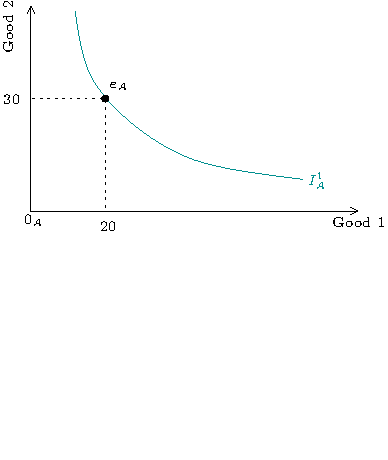
\includegraphics{pics/Edgeworth1}
\end{center}

\end{frame}


\begin{frame}
\frametitle{Trade between two people}
\begin{center}
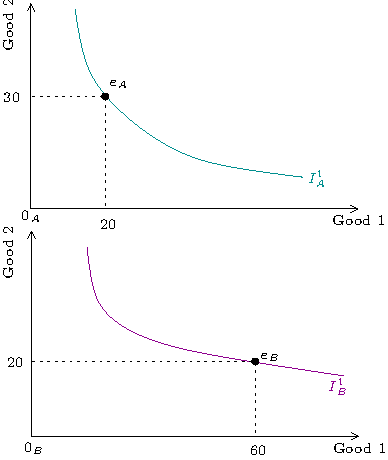
\includegraphics{pics/Edgeworth2}
\end{center}

\end{frame}

\begin{frame}
\frametitle{Trade between two people}
\begin{center}
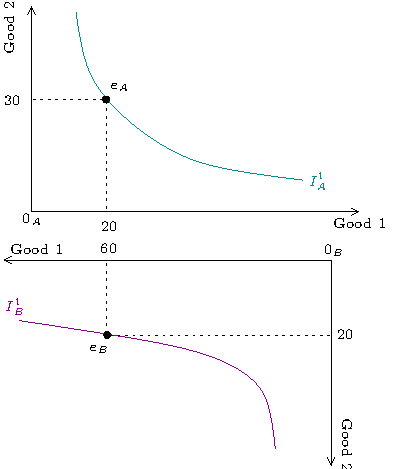
\includegraphics{pics/Edgeworth3}
\end{center}

\end{frame}

\begin{frame}
\frametitle{Trade between two people}
\begin{center}
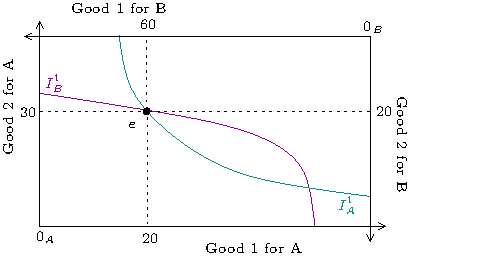
\includegraphics{pics/Edgeworth4}
\end{center}
Every possible allocation is associated with a unique point in this box!
\end{frame}


\begin{frame}
\frametitle{Mutually beneficial trades}
The usual assumptions on preferences:
\begin{enumerate}
\item Utility maximization
\item Convex indifference curves
\item More is better
\item No interdependence: I only care about my own bundle.
\end{enumerate}
\end{frame}



\begin{frame}
\frametitle{The Edgeworth Box}
\begin{center}
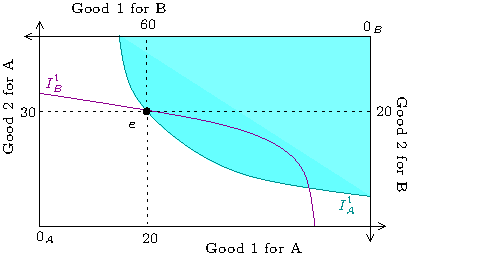
\includegraphics{pics/Edgeworth5}
\end{center}
These are the allocations that A prefers to $e$.
\end{frame}

\begin{frame}
\frametitle{The Edgeworth Box}
\begin{center}
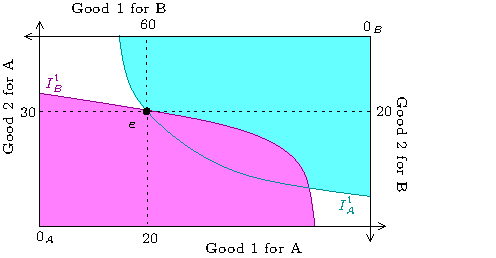
\includegraphics{pics/Edgeworth6}
\end{center}
These are the allocations that B prefers to $e$.
\end{frame}

\begin{frame}
\frametitle{The Edgeworth Box}
\begin{center}
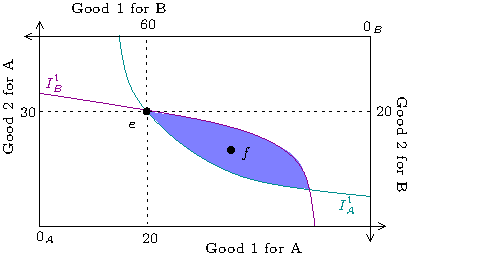
\includegraphics{pics/Edgeworth7}
\end{center}
Both A and B prefer $f$ to $e$.
\end{frame}

\begin{frame}
\frametitle{The Edgeworth Box}
\begin{center}
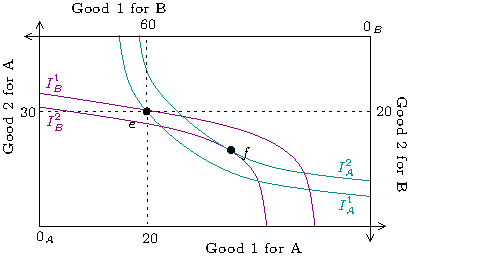
\includegraphics{pics/Edgeworth8}
\end{center}
Are there allocations that both A and B prefer to $f$?
\end{frame}


\begin{frame}
\frametitle{Pareto-efficient allocations}
Equivalent statements about allocation $f$:
\begin{enumerate}[<+->]
  \item The indifference curves of A and B are tangent at $f$.
  \item The MRS of A and B are the same at $f$.
  \item There are no mutually beneficial trades at $f$.
  \item $f$ is Pareto-efficient: to make on person better off, we need
    to make the other worse off.
\end{enumerate}
\uncover<5->{Are there are other such allocations?}
\bigskip

\uncover<6->{Many of them. The line through all of them is the \emph{contract curve.}}
\end{frame}

\begin{frame}
  \frametitle{The contract curve}
  \begin{center}
    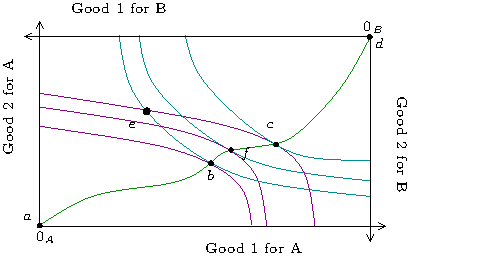
\includegraphics{pics/ContractCurve}
  \end{center}
\end{frame}

\begin{frame}
  \frametitle{Competitive exchange in the Edgeworth box}
  Which point should A and B choose on their contract curve?
  \bigskip

\uncover<2->{  If it's just the two of them, it depends on how they negotiate. But
  if there are many people like A and many like B, they might be price-takers.}
  \bigskip


\uncover<3->{  If price of good 1 is $p_1=\$2$ and the price of good 2 is
  $p_2=\$1$, then the relative price of good 1 in terms of good 2 is $\$\frac{1}{2}$.
}

  \bigskip
\uncover<4->{  At these prices, A and B will pick the allocation $f$.}

\end{frame}

\begin{frame}
  \frametitle{Competitive exchange in the Edgeworth box}
  \begin{center}
    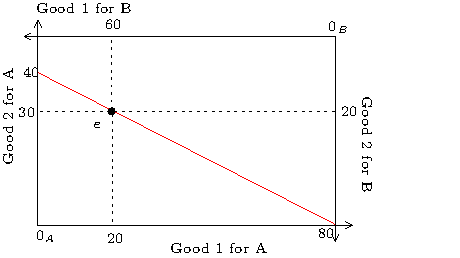
\includegraphics{pics/CompetitiveEq1}
  \end{center}
These prices give $A$ the red budget line. 
\end{frame}

\begin{frame}
  \frametitle{Competitive exchange in the Edgeworth box}
  \begin{center}
    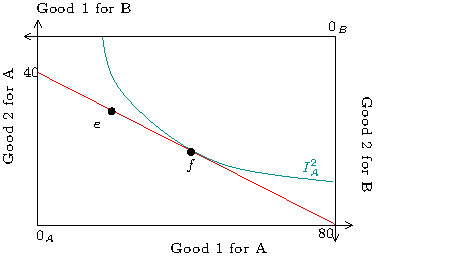
\includegraphics{pics/CompetitiveEq2}
  \end{center}
$A$ maximizes his preferences in this budget set.
\end{frame}

\begin{frame}
  \frametitle{Competitive exchange in the Edgeworth box}
  \begin{center}
    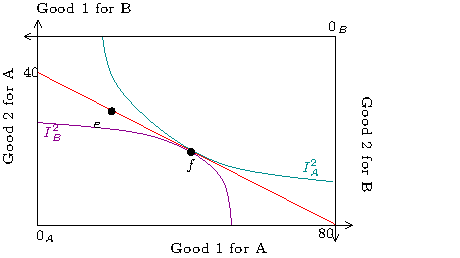
\includegraphics{pics/CompetitiveEq3}
  \end{center}
$B$ maximizes his preferences in his corresponding budget set.
\end{frame}

\begin{frame}
  \frametitle{Not all prices work though}
  \begin{center}
    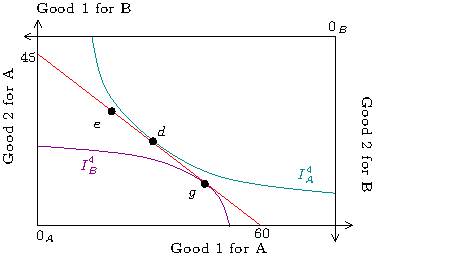
\includegraphics{pics/NoCompEq}
  \end{center}
A picks allocation $d$ but B picks allocation $g$.
\end{frame}


\begin{frame}
  \frametitle{Efficiency of competitive equilibrium}
  Since both A and B are maximizing their preferences:

  \[
  MRS_A = -\frac{p_1}{p_2} = MRS_B
  \]

\uncover<2->{Since $MRS_A = MRS_B$, the equilibrium allocation must be
Pareto-efficient!}
\bigskip

\uncover<3->{{First fundamental theorem of welfare economics:} \emph{Every
  competitive equilibrium allocation is Pareto-efficient.}}




\end{frame}


\begin{frame}
  \frametitle{Achieving other efficient allocations}
  What if we had a reason to want another allocation on the contract
  curve?
  \bigskip

\uncover<2->{  The initial distribution (endowment) determines which efficient
  allocation is obtained in equilibrium.}

  \bigskip
\uncover<3->{  If A starts with everything, the only competitive allocation is for
  him to end up with everything: no trade.}

  \bigskip
\uncover<4->{  Similarly, if B starts with everything, there is no trade.}

  \bigskip
\uncover<5->{  By varying the endowment, we can achieve anything in between.}

  \bigskip
\uncover<6->{  Second fundamental theorem of welfare economics: \emph{Any
    Pareto-efficient allocation can be obtained in equilibrium given
    the right endowment.}}

\end{frame}

\begin{frame}
  \frametitle{Efficiency and equity}
  Not all efficient allocations are ``fair'' in any reasonable sense.

\uncover<2->{  \bigskip
  The second theorem tells us that we can achieve other efficient
  allocations (which might be fairer) by redistributing endowments.}

  \bigskip
\uncover<3->{  Most government policies lead to some kind of redistribution.}

  \bigskip
\uncover<4->{  The Pareto-principle narrows down the set of allocations, but we
  need further criteria to get to a single allocation.}

  \bigskip
\uncover<5->{  When we move from one Pareto-efficient allocation to another, some
  people are better off while others are worse off.}



\end{frame}

\begin{frame}
  \frametitle{Picking an efficient allocation}
  When two allocations cannot be compared by the Pareto-criterion, we
  need another way.

\uncover<2->{  \bigskip
  We need a measure of how good an allocation is.}

\uncover<3->{    \bigskip One possible measure:
  \[W=CS+PS\]}


  \bigskip 
\uncover<4->{    Increasing $W$ is a ``sharper'' objective than just looking for a
  Pareto-improvement.}

  \bigskip
\uncover<5->{    A policy that maximizes $W$ does more than just find a
  Pareto-efficient allocation.}

\end{frame}

\begin{frame}
  \frametitle{Equity}
  There may be many Pareto-efficient allocations when two people
  trade.

\uncover<2->{  \bigskip
\emph{Utility possibility frontier:} the set of utility levels
corresponding to the Pareto-efficient allocations.}

\bigskip
\uncover<3->{   Use a social welfare function $W$ to measure how well off society is.
\[
W(u_1, u_2)
\]}

\bigskip
\uncover<4->{   We can also draw ``iso-welfare'' lines.}
\bigskip

\uncover<5->{   Higher iso-welfare lines correspond to higher social welfare.}
\end{frame}



\begin{frame}
  \frametitle{Equity}
  \begin{center}
    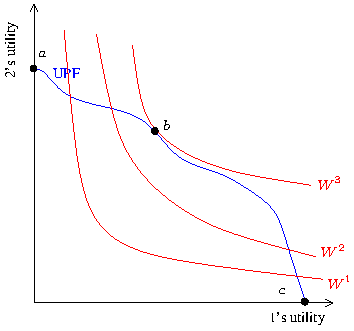
\includegraphics{pics/UPF1}
  \end{center}
If the $W$ has these iso-welfare lines, we pick $b$.\\
\
\end{frame}

\begin{frame}
  \frametitle{Equity}
  \begin{center}
    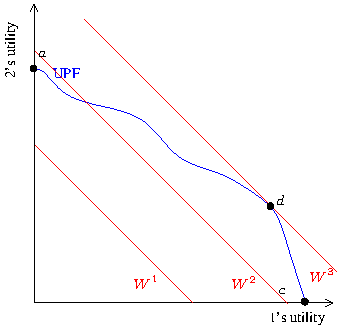
\includegraphics{pics/UPF2}
  \end{center}
The iso-welfare line has slope $-1$: we weight each individual's
utility equally.
\end{frame}


\begin{frame}
  \frametitle{Social welfare}
  Where does the social welfare function come from?
\bigskip

\uncover<2->{   In a democracy, people vote.}
\bigskip

\uncover<3->{   If a majority prefere $a$ to $b$ then $a$ is \emph{socially preferred}
to $b$.}

\bigskip
\uncover<4->{   Does this give us a well defined social preference?}

\bigskip
\uncover<5->{   Unfortunately not.}
\end{frame}


\begin{frame}
  \frametitle{Voting}
  \begin{tabular}{|l|c|c|c|}
    \hline & Individual 1  & Individual 2 & Individual3\\
\hline First choice & a & b & c \\
\hline Second choice & b & c & a \\
\hline Third choice & c & a & b \\
\hline
  \end{tabular}
\bigskip

\uncover<2->{When they vote:}
\uncover<3->{$a$ beats $b$}\uncover<4->{, $b$ beats $c$}\uncover<5->{, and
$c$ beats $a$!}
\end{frame}



\begin{frame}
  \frametitle{Arrow's Impossibility Theorem}
  Criteria for social decision making:
  \begin{enumerate}[<+->]
  \item  Social preference is complete and transitive.
  \item If everyone prefers $a$ to $b$, society prefers $a$ to $b$.
  \item Society's ranking of $a$ and $b$ depends only on how everyone
    feels about $a$ relative to $b$ (not how they rank other
    alternatives).
  \item No dictatorship: social preference shouldn't always reflect
    only one individual's preference,
  \end{enumerate}

\uncover<5->{The Theorem says that there is no such way of social decision making!}
\end{frame}


\begin{frame}
  \frametitle{Social welfare functions}
  \begin{enumerate}[<+->]
  \item  Utilitarianism: just add up everyone's utility.
    \[ W = u_1 + u_2 + \dots + u_n
    \]
    Notice that this may not lead us to anything resembling a fair allocation.
  \item Rawlsianism: society is only as well off as its worst member.
    \[
    W = \min\{u_1, u_2,\dots, u_n\}
    \]
  \end{enumerate}

  
\end{frame}















\end{document}








